% !TEX program = pdflatex
%%%%%%%%%%%%%%%%%%%%%%%%%%%%%%%%%%%%%%%%%
% Structured General Purpose Assignment
% LaTeX Template
%
% This template has been downloaded from:
% http://www.latextemplates.com
%
% Original author:
% Ted Pavlic (http://www.tedpavlic.com)
%
% Note:
% The \lipsum[#] commands throughout this template generate dummy text
% to fill the template out. These commands should all be removed when
% writing assignment content.
%
%%%%%%%%%%%%%%%%%%%%%%%%%%%%%%%%%%%%%%%%%

%----------------------------------------------------------------------------------------
%	PACKAGES AND OTHER DOCUMENT CONFIGURATIONS
%----------------------------------------------------------------------------------------

\documentclass{article}

\usepackage{fancyhdr} % Required for custom headers
\usepackage{lastpage} % Required to determine the last page for the footer
\usepackage{extramarks} % Required for headers and footers
\usepackage{graphicx} % Required to insert images
\usepackage{subcaption}
\usepackage{lipsum} % Used for inserting dummy 'Lorem ipsum' text into the template

\usepackage[utf8]{inputenc}
\usepackage[ngerman,english]{babel}
\usepackage[T1]{fontenc}
\usepackage{breakurl}
\usepackage[hyphens]{url}
\usepackage{color}
\usepackage{float}
\usepackage[hidelinks]{hyperref}
\usepackage{tabularx}
\usepackage{enumitem}
\usepackage{color, colortbl}
\usepackage[super]{nth}
\usepackage{wrapfig}
\usepackage{amsmath}

\usepackage[
	backend=biber,
	style=numeric-comp,
	natbib=true,
	url=false,
	doi=false,
	eprint=false,
	sorting=none,
	isbn=false]
	{biblatex}

\bibliography{references}

\addto\captionsenglish{%
  \renewcommand{\contentsname}%
    {Table of Contents}%
}

% Margins
\topmargin=-0.45in
\evensidemargin=0in
\oddsidemargin=0in
\textwidth=6.5in
\textheight=9.0in
\headsep=0.25in

\linespread{1.1} % Line spacing
% Set up the header and footer
\pagestyle{fancy}
\lhead{} % Top left header
\chead{} % Top center header
\rhead{\firstxmark} % Top right header
\lfoot{\lastxmark} % Bottom left footer
\cfoot{} % Bottom center footer
\rfoot{Page\ \thepage\ of~\pageref{LastPage}} % Bottom right footer
\renewcommand\headrulewidth{0.4pt} % Size of the header rule
\renewcommand\footrulewidth{0.4pt} % Size of the footer rule

\setlength\parindent{0pt} % Removes all indentation from paragraphs

\begin{document}
\setcounter{tocdepth}{2} % No subsubsections


%----------------------------------------------------------------------------------------
% TITLE PAGE
%----------------------------------------------------------------------------------------
\pagenumbering{gobble}
% \maketitle
\begin{titlepage}
  \centering
\includegraphics[width=5cm]{figures/tumlogo}

  \vspace{2.5cm}
  \Huge{Advanced Computer Networking} \\
  \vspace{0.1in}\huge{Summary}\\

  \Large
  \vspace{1.5cm}
  \begin{tabularx}{9cm}{r l}
    Author: & Thomas Pettinger\\
  \end{tabularx}

  \vfill
  \textbf{2017--03--03} \\
  \vspace{0.3in}\normalsize{Advanced Computer Networking}\\
  \vspace{0.03in}\normalsize{\textsc{Technische Universität München}}\\
  \vspace{1cm}

\end{titlepage}
%----------------------------------------------------------------------------------------


\newpage
\thispagestyle{empty}
\tableofcontents

\newpage
\pagenumbering{arabic}

%!TEX root = ../report.tex

\section{Introduction}
Terminology:
\begin{description}
  \item[Protocols] control sending and receiving of messages
  \item[Internet] loosely hierarchical global network
  \item[Internet Standards]\hfill
    \begin{itemize}
      \item RFC:\@ Request for comment
      \item IETF:\@ Internet Engineering Task Force
      \item IANA:\@ Internet Assigned Numbers Authority
    \end{itemize}
\end{description}

\subsection{Protocols}
Protocols take care of addressing, fragmentation \& re-sequencing, error control, congestion control, compression, privacy and more.

The internet has an layered architecture of protocols.
On the sender side, protocols take the PDU (Protocol Data Unit) from layer N+1, add their header and trailer and pass the SDU (Service Data Unit) to layer N-1.
On the receiver side, the corresponding protocol takes the PDU from layer N-1, strips header and trailer again and passes the SDU to layer N+1.
\begin{figure}[H]
  \centering
  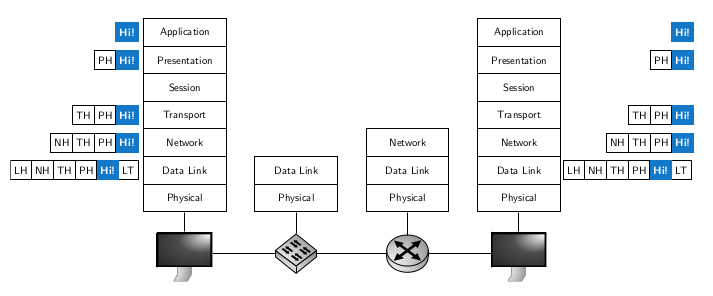
\includegraphics[width=.6\textwidth]{figures/internet_layering.png}
  \caption{Internet Layers}
\end{figure}

Protocol layering is necessary because one does not want to implement everything to the physical layer when writing a networking application.
On the other hand, layering also introduces some problems like protocol layers are sometimes reusing techniques of other layers like ARQ (Automatic Repeat Query) and layers might need informations of other layers.

\subsection{Node Forwarding Performance}
During transmission, packets might get delayed or even lost for several reasons.
First, the packets need some time to get written to router buffers, secondly the packet arrival rate might exceed the output link capacity and lastly the packets need to wait again for being sent from the packet queue in routers.

The sources for these delays are listed below.
\begin{enumerate}
  \item Processing delay: interrupt handling when receiving new packets and processing for further transmission
  \item Queuing delay: waiting time in output queue
  \item Transmission delay: time to send bits into link: $= \frac{\text{packet length L (bit)}}{\text{link bandwidth (bps)}}$
  \item Propagation delay $=\frac{\text{length of physical link d}}{\text{propagation speed} \approx 2 \cdot 10^8 m/s}$
\end{enumerate}
The total amount of delay is then $d_{nodal} = d_{proc} + d_{queue} + d_{trans} + d_{prop}$

To reduce total packet delays for a connection consisting of several links one can use circuit switching, where packets do not have to be received entirely to be sent to the next link.
Another alternative is to split packets into (very) small sub-parts (= segmenting) and using pipelining (parallel computing of packets).

\newpage

%!TEX root = ../report.tex

\section{Link Layer}

\newpage

%!TEX root = ../report.tex

\section{Network Layer}
The network layer serves the following functions:
\begin{itemize}
  \item IP protocol for addressing, datagram format and packet handling conventions
  \item Routing protocols for path selection
  \item ICMP protocol for error reporting and router signaling
\end{itemize}

\subsection{Internet Protocol}
\begin{figure}[H]
  \centering
  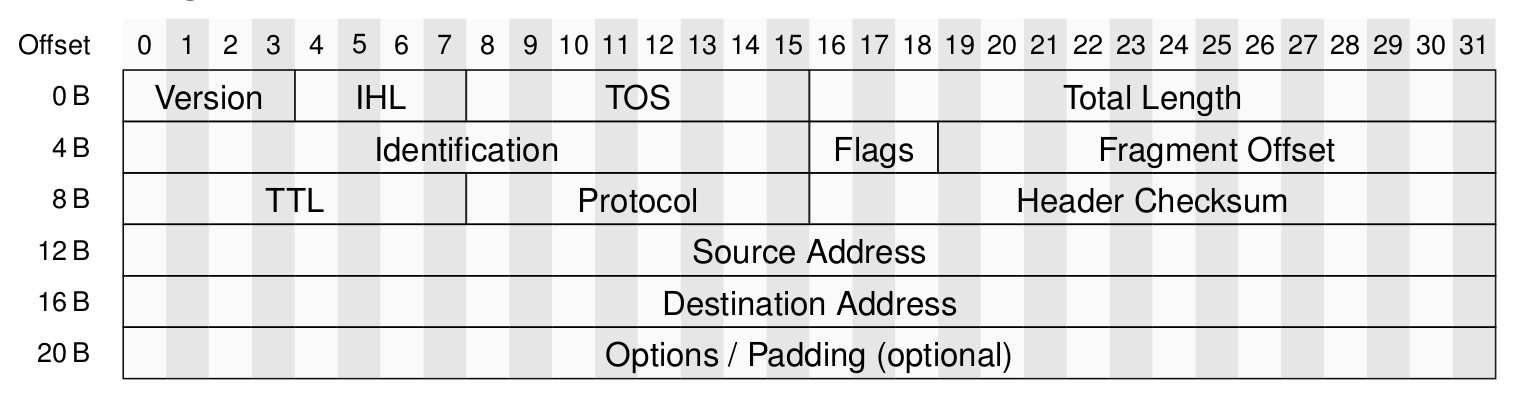
\includegraphics[width=.8\textwidth]{figures/ipv4_datagram.png}
  \caption{IPv4 Datagram}\label{fig:ipv4_datagram}
\end{figure}

\subsubsection*{IPv4 Addressing}
IPv4 addresses are 32-bit identifiers for every host and router interfaces where interfaces represent the connection between host/router and physical link.

Subnets are device interfaces with the same subnet part of the IP address which can physically reach each other without intervening router.

Splitting the IP address into network and host part is done in the following way (for the address 192.168.128.1/17):
\begin{figure}[H]
  \centering
  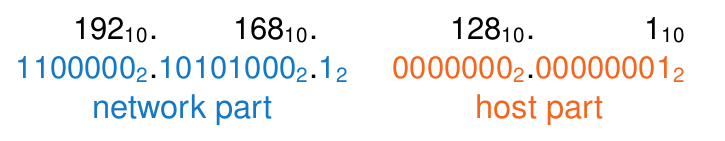
\includegraphics[width=.6\textwidth]{figures/ip_split.png}
\end{figure}

From 1982 to 1993, IP addresses were classfully divided as shown in Figure~\ref{fig:classful_ips}.
\begin{figure}[h]
  \centering
  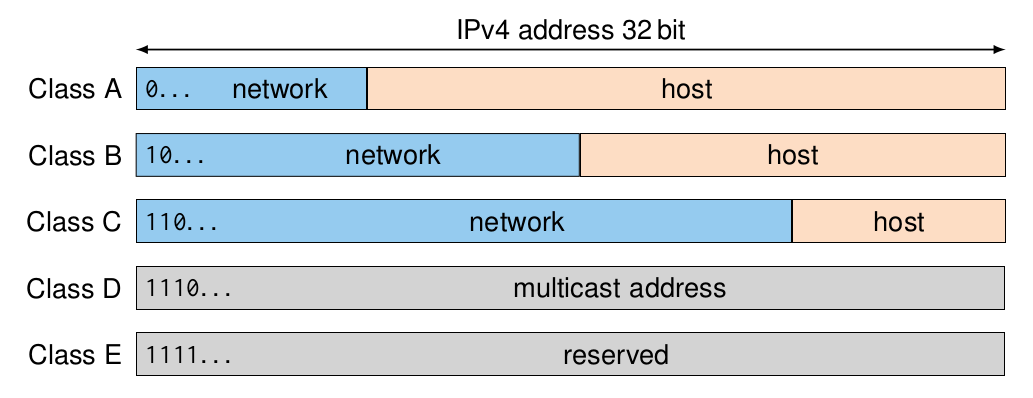
\includegraphics[width=.8\textwidth]{figures/classful_ip.png}
  \caption{Classful IPs}\label{fig:classful_ips}
\end{figure}
In 1993, Classless Inter-Domain Routing (CIDR) was introduced which allowed arbitrary subnet length.
To route packets, prefix matching is used which checks which entry in the routing table fits best for the incoming packet's network prefix.

\subsection{ICMP}
The Internet Control Message Protocol (ICMP) are located above IP but can be considered as part of the IP layer.
It is used for communicating error messages and other attention requiring conditions for IP and TCP or UDP\@.
Two classes of ICMP messages are possible:
\begin{enumerate}
  \item Query messages: only kind that generates other ICMP messages
  \item Error messages: contain IP header and first 8 bytes (today as much as possible up to 572 bytes) of datagram that caused the ICMP message which allows the receiver to put it into context
\end{enumerate}
The structure of an ICMP message is shown in Figure~\ref{fig:icmp_message}.
\begin{figure}[H]
  \centering
  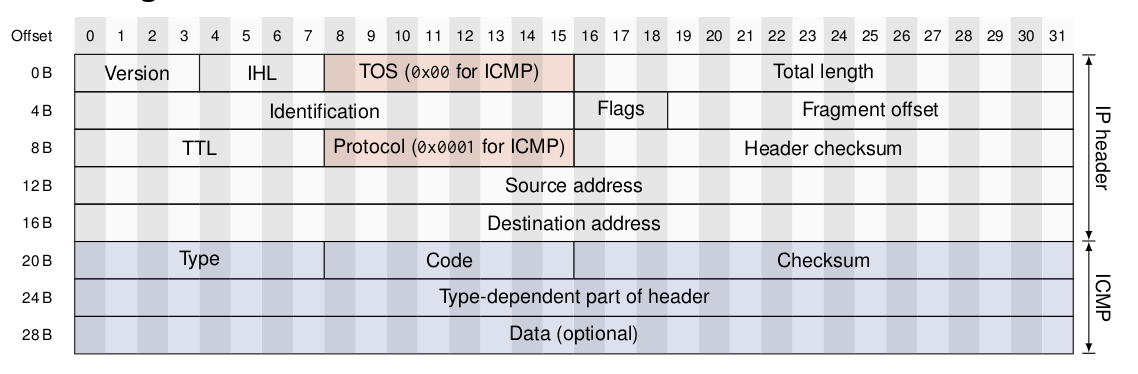
\includegraphics[width=.8\textwidth]{figures/icmp_message.png}
  \caption{ICMP Message}\label{fig:icmp_message}
\end{figure}


\newpage

%!TEX root = ../report.tex

\section{Structure of the Internet}
The Internet is separated into regions called \textbf{autonomous systems (AS)}.
Routers in the same AS use \textbf{intra-AS routing} protocols whereas routers connecting different ASes, called \textbf{gateway/border routers} use \textbf{inter-AS routing} protocols.
\textbf{Transit domains} are ASes, that forward traffic from one AS to another where in contrast a \textbf{stub domain} is an AS without transit traffic.
Internet service providers are divided hierarchically: Tier-1 providers are on the top level and connected to each other.
They can send traffic to one another without paying (peering).
Tier-2 providers are connected to one or multiple Tier-1 providers and possibly to other Tier-2 providers.
Tier-3 providers and local ISPs then are the last hop to the end systems.
Every ISP has its own IP range purchased at the regional Internet Registrars which they are able to divide amongst their customers.

\subsection{Associations of Internet Names and Numbers}
\begin{description}
  \item[ICANN] Internet Corporation for Assigned names and numbers: Administration of DNS TLDs
  \item[IANA] Internet Assigned Numbers Authority: Assignment of Internet Numbers, administration of DNS root name servers and reverse DNS infrastructure, Assignment of protocol names and numbers
  \item[NRO] Number Resource Organization: Association of the 5 Regional Internet Registrars (RIR)
  \item[Regional Registras] Assigns IP addresses and AS numbers, administration of local Internet Registers (LIR)
  \item[RIPE] Registration and administration of Internet resources: AS, prefix and routing information
\end{description}

\subsection{Routing Algorithms}
Routing algorithms are usually an applied approach of least-cost path search in weighted graphs.
The costs are represented for example by the inverse link bandwidth.

They can be classified by several criteria:
\begin{itemize}
  \item Global or decentralized
  \begin{itemize}
    \item Global/Link State algorithms (L-S): All routers know the graph topology and link costs (usually through broadcasts) and are able to calculate the routing table by themselves (usually via Dijkstra)
    \item Decentralized/Distance Vector algorithms (D-V): Routers only know neighbours and link costs to neighbours, routing tables are computed in collaboration
  \end{itemize}
  \item Static or dynamic
  \begin{itemize}
    \item Static: Routes change slowly over time
    \item Dynamic: Routes change more quickly due to periodic update and in response to link cost changes
  \end{itemize}
  \item Scope: Intra- vs Inter- vs special purpose
  \item Type of traffic: Unicast vs multicast
  \item Trigger type: permanent routing vs on-demand routing (create routing table only if necessary)
\end{itemize}

\subsubsection*{D-V Algorithm}
A typical example for a distance vector algorithm is the Bellman-Ford algorithm:
\begin{enumerate}
  \item Define $D_x(y)$ as the estimate of the least cost from x to y
  \item Node x knows all costs to each neighbour v: $c(x,v)$
  \item Every node x maintains a distance vector $D_x = [D_x(y): y \in N]$ where N is the set of nodes
  \item Node x also maintains the distance vectors for each neighbour $D_v = [D_v(y): y \in N]$
  \item Update messages for the estimated distances are sent from time to time to neighbours and might lead those to update its own distance vectors according to the B-F equation:
    $D_x(y) \leftarrow \min_v{c(x,v) + D_v(y)} \text{ for each node } y \in N$
  \item Under minor, natural conditions these estimates of $D_x(y)$ to the actual least costs $d_x(y)$
\end{enumerate}

A problem which occurs with this approach is that if a link becomes unavailable and thus its cost infinity, the algorithm will encounter the count to infinity problem.
The paths to the disconnected node are increased per update by one, infinitely.
Solutions for this are
\begin{itemize}
  \item Finite infinity: set infinite costs to a specific number, e.g. 16 in RIP
  \item Split Horizon: Tell neighbours that they are part of the best path to a destination that the destination cannot be reached from the original node
  \item Poisoned Reverse: Actively adverse a route as unreachable to neighbours from which the route was learned
\end{itemize}

\subsubsection*{Path Vector Protocols}
Path vector protocols try to improve the fact of D-V protocols that they do now include topology information.
For each destination, the entire path for each destination is told to neighbours and then the cost calculation is done by looking at the paths.
Furthermore loop detection can easily be done by searching if the own node ID appear in the paths.
PV protocols are quite rarely used though, mainly in BGP but that is much more complex than just paths.

\subsubsection*{Intra-AS Routing/Interior Gateway Protocols (IGP)}
\begin{enumerate}
  \item RIP: Routing Information Protocol
  \item OSPF: Open Shortest Path First (hierarchical LSA), usually in medium to large systems
  \item IS-IS: Intermediate System to Intermediate System, medium-sized ASes
  \item (E)IGRP: (Enhanced) Interior Gateway Routing Protocol, CISCO proprietary, hybrid of LS and DV
\end{enumerate}
\vspace{5pt}

The open shortest path first protocol (OSPF) uses an link state algorithm to generate routing tables.
Advertisement of topology and costs of the directed graph is done via advertisement flooding.
All messages are authenticated to prevent malicious intrusion (e.g.\ with IPsec).
Furthermore multiple same-cost paths are supported and different metrics are considered to define the costs for links.
The protocol has integrated unicast and multicast support (Multicast OSPF) that uses the same topology database as OSPF which lowers traffic.
To even further reduce the traffic, hierarchical OSPF can be used in large domains where a two-level hierarchy is created.
On the one side the backbone which are running OSPF among themselves and on the other hand local areas.
Area border routes summarize distances to networks in the own area and advertises them to other area border routers.

\subsubsection*{Inter-domain routing}
Inter domain routing is almost exclusively handled with the Boarder Gateway Protocol (BGP).
It provides means to obtain subnet reachability from neighbouring ASes (external BGP, eBGP), propagate that information in the AS internally (internal BGP, iBGP) and determine good routes according to that information and router policies via semi-permanent TCP connections.
ASes advertise reachable network prefixes to others and give a promise to forward traffic to that IP address space.
These advertisements include a multitude of BGP attributes like AS-Paths (Path of AS-Numbers the advertisement has passed through) or the Next-Hop (gateway router to the next-hop AS).

BGP messages can have the following types:
\begin{itemize}
  \item OPEN: open a BGP session
  \item NOTIFICATION: error occurred, close BGP session
  \item KEEPALIVE: null data to prevent closing of TCP session
  \item UPDATE: about changed routes, also removed routes\\
    These messages consist of the destination IP prefix, the AS path and the next hop and other attributes related to local preferences, route origins or others.
    Routers than can make routing decisions based on this information and their policies.
\end{itemize}

Routers may learn about multiple routes for a prefix.
If that is the case, one of those routes has to be selected due to criteria like an policy decision, shortest AS-Path or closest next hop (hot-potato-routing) amongst others.\\
\vspace{5pt}

In the context of inter-domain routing, we define the following \textbf{terminology}:
\begin{description}
  \item[Transit AS] Relays traffic between other ASes
  \item[Stub AS] Buys transit from one other AS but does not offer transit
  \item[Multi-homed AS] Buys transit from $\geq 2$ other ASes, does not offer transit
  \item[Peering] having a BGP relationship
    \begin{itemize}
      \item Private peering: peering between ASes in private locations like ASes or neutral server rooms
      \item Public peering: "official" peering locations ("Room full of switches") like in Frankfurt or London
    \end{itemize}
  \item[Provider] Offers transit traffic for receiving money
  \item[Customer] Gets transit for paying money
  \item[Siblings] Mutual transit agreement to provide connectivity of the rest of the Internet for each other, so kind of an very extensive peering
\end{description}

\subsubsection*{Business and Policy Routing}
Routing is done by the policy
\begin{equation*}
  \text{Routes via customer > Routes via peer > routes via provider}
\end{equation*}
In route announcement on the other hand first announce routes that incur financial gain if others use them, then routes that reduce costs if others use them and especially do not advertise routes that incur financial loss as long as an alternative exists.
ASes might add the same AS number subsequently to an AS-Path to increase path costs if they prefer another connection over the one this announcement was sent, might be due to lower costs.

\subsubsection*{Tiers and Default-Free-Zone}
Like mentioned in the introduction to this chapter, different tiers of providers exist.
With our definitions in inter-domain routing of costumers, providers and peering, we can now better define them:
\begin{description}
  \item[Tier-1/Default-Free-Zone (DFZ)] Only have customers and peers, no providers
  \item[Tier-2] only peerings and only tier-1 providers
  \item[Tier-n] at least noe tier-(n-1) provider
\end{description}

\subsubsection*{Internet Fixed Points}
Internet fixed points are ASes that are stable over a long period of time from different perspectives.
Together these form the so called backbone of the Internet.
To find those fixed points, the \textbf{k-core algorithm} can be applied:
\begin{enumerate}
  \item Remove all nodes with $degree = 1$ so long until no degree 1 nodes are left
  \item Remove all nodes with $degree = 2$ so long until no degree 2 nodes are left
  \item Do this until no nodes left $\Rightarrow$ $(Steps - 1)-core$ found.
\end{enumerate}

\newpage

% Needs to be enabled when there are any references.
% \clearpage
% \addcontentsline{toc}{section}{\refname}
% \printbibliography

\end{document}
